\section{Specification and Design}
\label{sec:design}

\subsection{Pure logic is separated from hardware, and the board decides everything}
Table~\ref{tab:arch} divides the system. \code{game.c} and \code{server.c} contain no HAL or CMSIS calls, so the
identical files are compiled for the Cortex-M0 and for the PC test builds; only \code{uart.c}, \code{main.c}
and the button/LED code touch registers. The server owns the board, the turn, legality, win detection, the computer opponent's moves and
the reply text. The client owns only presentation (drawing, score, sound) and the timing of its own requests. It never
computes a legal move or a winner, so a buggy or hostile client can at worst be refused.

\begin{table}[t]
\centering
\caption{Modules and who owns each decision.}
\label{tab:arch}
\scriptsize
\begin{tabular}{@{}L{1.9cm}L{1.0cm}L{4.9cm}@{}}
\toprule
Module & HAL? & Responsibility \\
\midrule
\code{game.c} & no & 10-byte state, validate-then-commit, 8-line win test \\
\code{server.c} & no & byte-driven framer, parser, checksum, dispatch to \code{game.c} \\
\code{ai.c} & no & minimax opponent for O; only picks a cell, the move goes through \code{game.c} \\
\code{uart.c} & yes & USART1 RX interrupt, 128-byte ring, polled TX \\
\code{main.c} & yes & loop: drain ring, \code{server_rx}, \code{server_tick}, button, LED \\
\code{client.py} & no & protocol client, checksum check, \code{GameView} (no Tk) \\
\code{app.py} & Tk & canvas, worker thread, score, sound \\
\bottomrule
\end{tabular}
\end{table}

\subsection{The server FSM validates before it commits}
Figure~\ref{fig:fsm} shows the three states. IDLE accepts \code{CONNECT}, \code{NEW} and \code{DISCONNECT}. IN\_PROGRESS accepts
\code{MOVE}, \code{STATE} and \code{RESIGN}, and GAME\_OVER accepts \code{NEW}, \code{STATE} and \code{DISCONNECT}. The \code{MOVE}
branch runs the checks range, turn, occupancy in that order, each with its own NACK exit that returns to IN\_PROGRESS
without writing. Only a move passing all three is committed; the win or draw test then decides between IN\_PROGRESS and
GAME\_OVER. The button resets to IDLE from any state. The figure omits the framer errors, which never reach the FSM
(Table~\ref{tab:framing}).

\begin{figure*}[t]
\centering
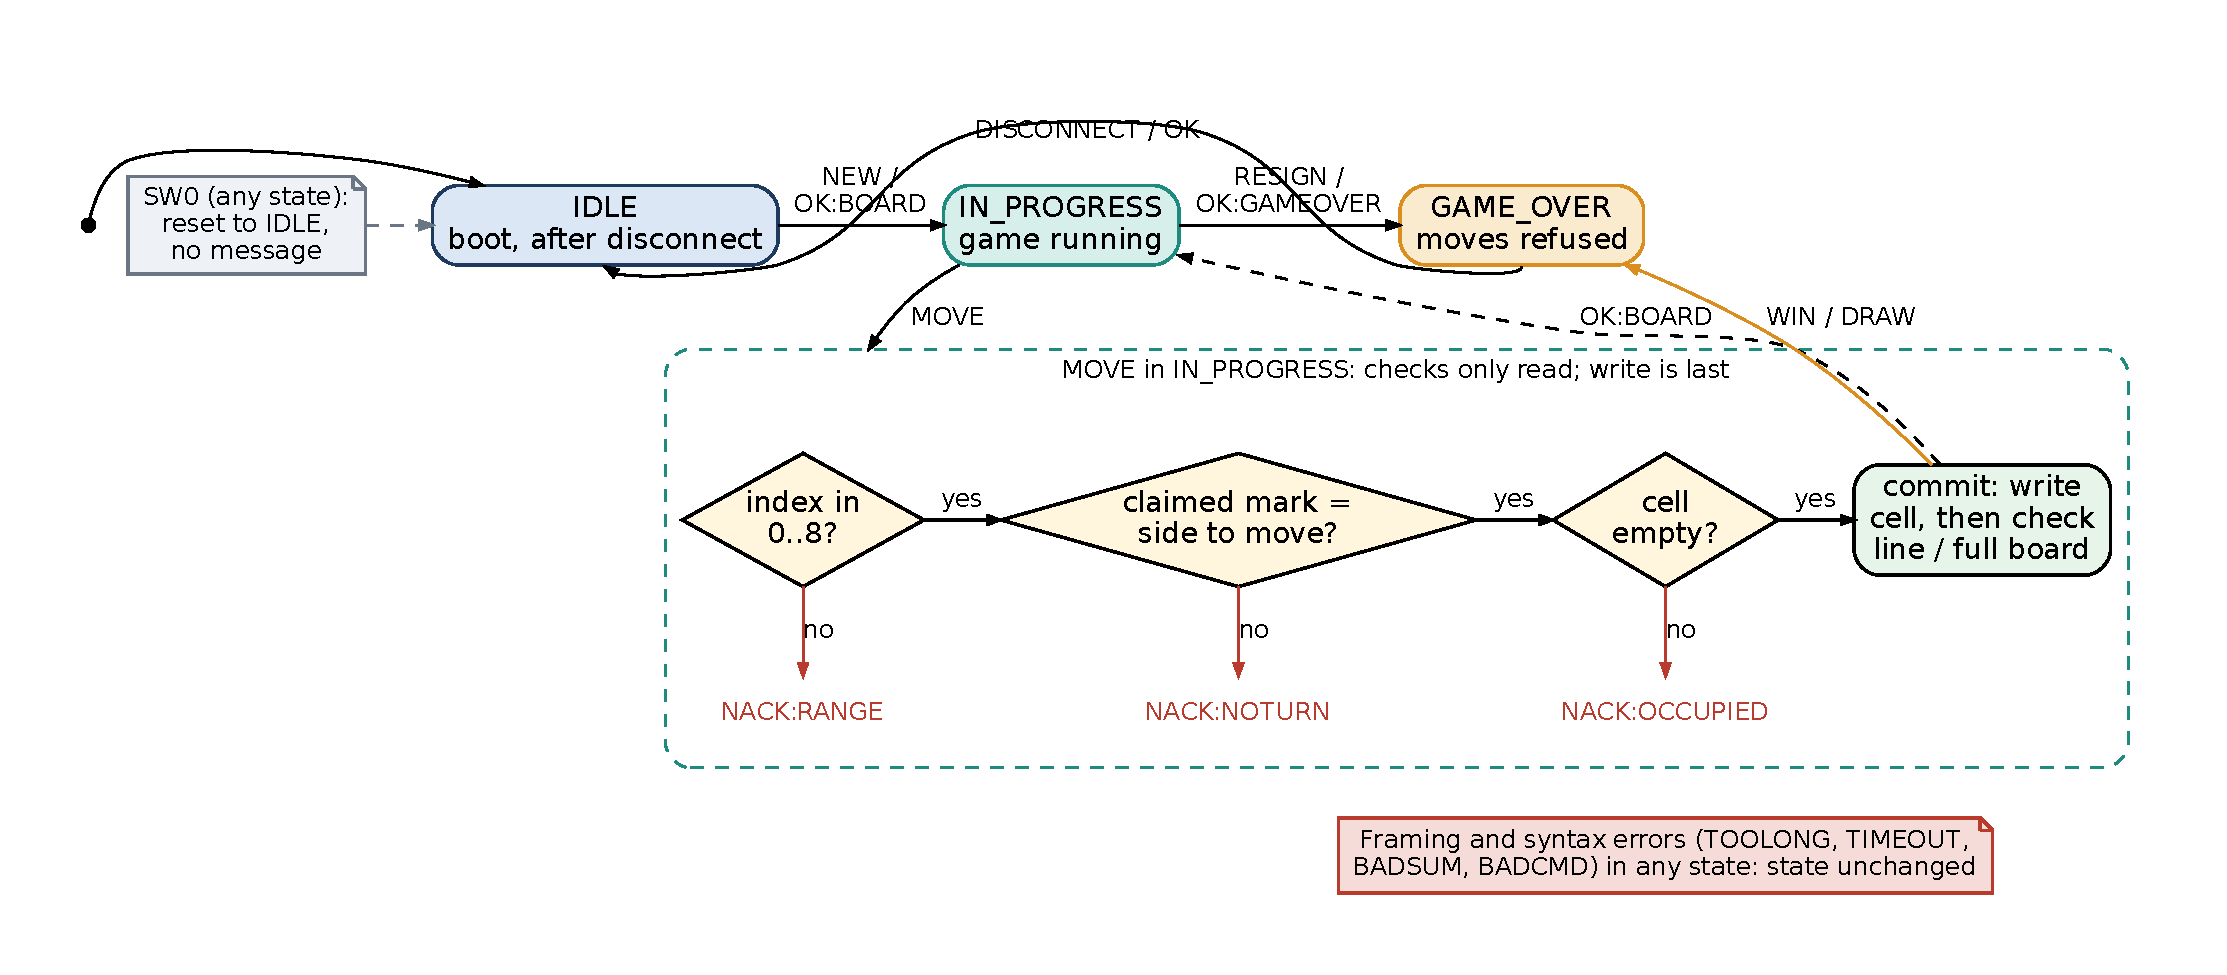
\includegraphics[width=\textwidth]{figures/fsm.pdf}
\caption{Server FSM with the \code{MOVE} validation branch. Transitions read ``command [guard] / reply''.}
\label{fig:fsm}
\end{figure*}

\subsection{The GUI never draws before the server confirms}
Figure~\ref{fig:gui} shows the client flow. A request is placed on a worker thread, so the Tk main loop never waits on the serial
port, and the main loop polls a result queue every 30~ms. On a reply the client first verifies the checksum; a missing or wrong
one counts as not received. Only a verified \code{OK:BOARD}, \code{WIN}, \code{DRAW} or \code{BOARD} reply redraws the
board, and a NACK shows its message and leaves the display as it was. A click on an occupied cell is sent anyway, so the board's \code{NACK:OCCUPIED} is what the user sees: the GUI does not decide legality. After a win, draw or resign, cells are disabled until
\code{NEW}. On a lost reply (1~s timeout) the client sends \code{STATE} once and redraws from it, because \code{STATE} is safe
to repeat; if that also fails it reports ``server not responding''. If a \code{MOVE} is answered \code{NACK:NOGAME}
mid-game, the board was reset by its button, so the client returns to the start screen.

\begin{figure*}[t]
\centering
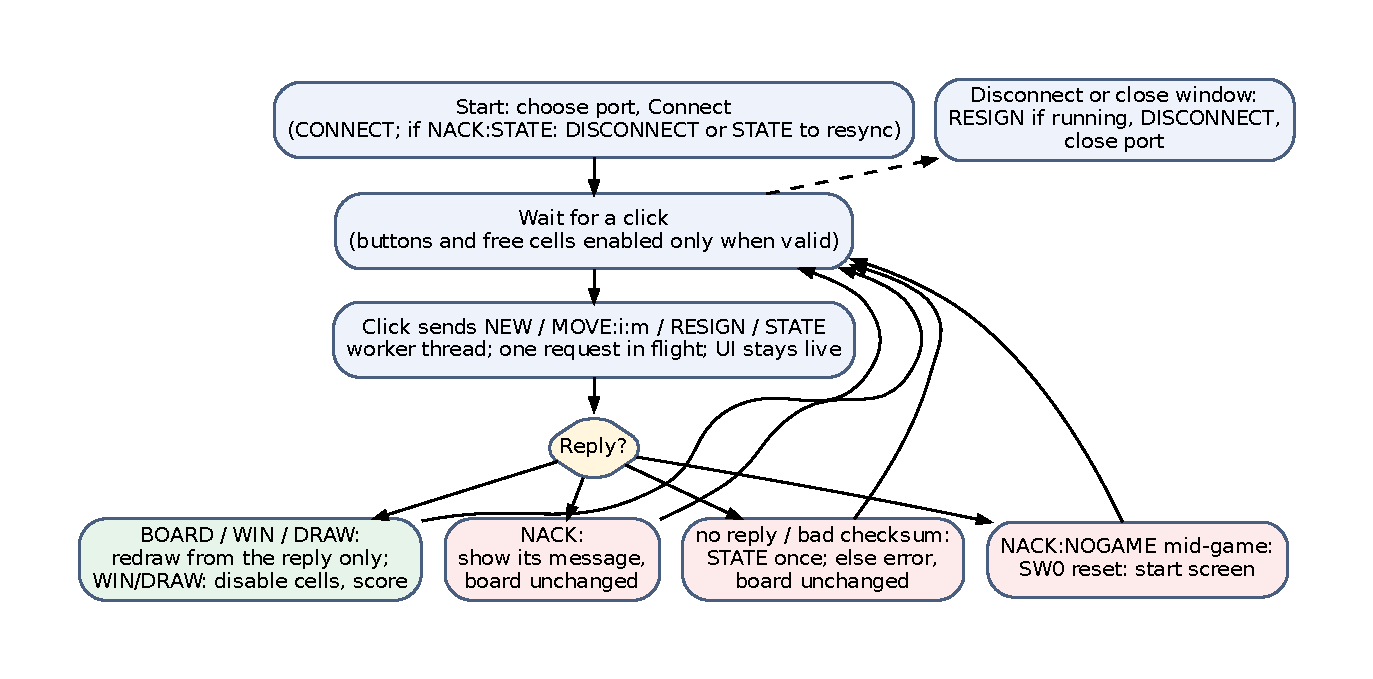
\includegraphics[width=0.78\textwidth]{figures/gui_flow.pdf}
\caption{GUI flowchart: requests run on a worker thread and the display changes only on a verified reply.}
\label{fig:gui}
\end{figure*}

\subsection{The USB cable is the UART link; SW0 and the LED are local}
Figure~\ref{fig:circuit} shows the connection. No adapter is used: the on-board ST-Link bridges USART1 to a USB virtual COM
port, with TX on PA9 and RX on PA10 (alternate function AF1, datasheet Table~14~\cite{ds8668}). SW0 on PA0 is active low with
the internal pull-up; a press resets the game to IDLE. The red LED is on PB10 and the green on PB11, each through 150~$\Omega$
(schematic~\cite{schematic}). The LED is off in IDLE, green while X is to move, red while O is to move, and both blink together
at 2~Hz (250~ms half-period in code) in GAME\_OVER.

\begin{figure}[t]
\centering
\resizebox{\linewidth}{!}{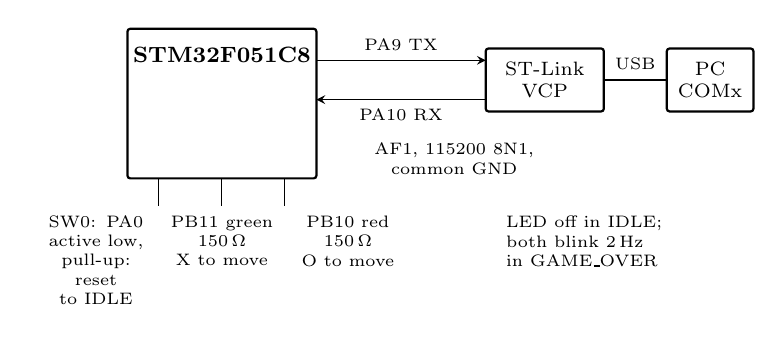
\begin{tikzpicture}[x=1cm,y=1cm,font=\scriptsize,
  box/.style={draw,thick,rounded corners=1pt,align=center,inner sep=2pt}]
 \node[box,minimum width=2.4cm,minimum height=1.9cm] (mcu) at (0,0) {};
 \node[font=\footnotesize\bfseries] at (0,0.62) {STM32F051C8};
 \node[box,minimum width=1.5cm,minimum height=0.8cm] (stl) at (4.1,0.3) {ST-Link\\VCP};
 \node[box,minimum width=1.1cm,minimum height=0.8cm] (pc) at (6.2,0.3) {PC\\COMx};
 \draw[->,>=stealth] (1.2,0.55) -- node[above,font=\fontsize{6}{7}\selectfont]{PA9 TX} (3.35,0.55);
 \draw[<-,>=stealth] (1.2,0.05) -- node[below,font=\fontsize{6}{7}\selectfont]{PA10 RX} (3.35,0.05);
 \draw[thick] (4.85,0.3) -- node[above,font=\fontsize{6}{7}\selectfont]{USB} (5.65,0.3);
 \node[font=\fontsize{6}{7}\selectfont,align=center] at (2.95,-0.7) {AF1, 115200 8N1,\\common GND};
 \foreach \x/\t in {-1.6/{SW0: PA0\\active low,\\pull-up: reset\\to IDLE}, 0/{PB11 green\\150\,$\Omega$\\X to move}, 1.6/{PB10 red\\150\,$\Omega$\\O to move}}{
   \draw (\x*0.5,-0.95) -- (\x*0.5,-1.3);
   \node[below,align=center,text width=1.5cm,font=\fontsize{6}{7}\selectfont] at (\x,-1.3) {\t};}
 \node[align=left,font=\fontsize{6}{7}\selectfont] at (4.6,-1.75) {LED off in IDLE;\\both blink 2\,Hz\\in GAME\_OVER};
\end{tikzpicture}
}
\caption{UART path to the PC and the button and LED pins.}
\label{fig:circuit}
\end{figure}
